\documentclass[t]{beamer}

% Load general definitions
% Preamble file - general definitions, package loading, etc.

%=================================
% Load packages
\usepackage{amssymb,amsmath}
\usepackage{graphicx}
\usepackage{url}
\usepackage{tikz}
\usetikzlibrary{mindmap,trees,arrows}
\usepackage{fancyvrb}
\usepackage[portuguese]{babel} 
\usepackage[utf8]{inputenc}
\usepackage{subfigure}
\usepackage{times}
\usepackage[T1]{fontenc}
\usepackage{cancel}
\usepackage{color}
\usepackage{listings}
\usepackage[document]{ragged2e}
\usepackage{hyperref}
\usepackage{listings}


%=================================
% Set mode
\mode<presentation>
{
	\usetheme{Madrid}
	\usecolortheme{structure}
	\useoutertheme{infolines}
	\setbeamercovered{invisible}
}

% Get rid of nav bar
\beamertemplatenavigationsymbolsempty

% Insert frame number at bottom of the page.
\usefoottemplate{\hfil\tiny{\color{black!90}\insertframenumber}} 

%=================================
% Define new commands

\newcommand\Real{{\mathbb{R}}}
%\newcommand{\vi}{\vspace{0.6\baselineskip}}
%\newcommand{\goodgap}{\hspace{\subfigtopskip}\hspace{\subfigbottomskip}}


% Equation environments
\newcommand{\beq}{\begin{equation}}
\newcommand{\eq}{\end{equation}}
\newcommand{\beqs}{\begin{equation*}}
\newcommand{\eqs}{\end{equation*}}
\newcommand{\beqn}{\begin{eqnarray}}
\newcommand{\eqn}{\end{eqnarray}}
% Bold variables
\newcommand{\mbf}[1]{\ensuremath{\mathbf{#1}}}
% Itemization
\newcommand{\bitem}{\begin{itemize}}
\newcommand{\eitem}{\end{itemize}}
\newcommand{\spitem}{\vskip 1em\item}
\newcommand{\bitems}{\begin{itemize}\item}
\newcommand{\benums}{\begin{enumerate}\item}
\newcommand{\eenum}{\end{enumerate}}
% color blocks
\newenvironment{colorblock}[2]{%
\setbeamercolor{block title}{#2}
\begin{block}{#1}}{\end{block}}
% Vertical spacing
\newcommand{\vone}{\vskip 1em}
\newcommand{\vhalf}{\vskip .5em}
% Frame environments
\newenvironment{ftst}[3][t]{%
\begin{frame}{environment=ftst,#1}
\frametitle{#2}
\framesubtitle{#3}}{\end{frame}}
\newenvironment{ftstf}[2]{
\begin{frame}[fragile,environment=ftstf]
\frametitle{#1}
\framesubtitle{#2}}{\end{frame}}
% colors
\definecolor{MyGray}{rgb}{0.5,0.5,0.5}
\definecolor{MyDBGray}{rgb}{0.1,0.1,0.4}
\definecolor{darkgreen}{rgb}{0,0.4,0}
\definecolor{black}{rgb}{0,0,0}
\def\defn#1{{\color{red} #1}}
% Footnote
\renewcommand{\thefootnote}{\alph{footnote}}
% Relaxed footnotes
\newcommand{\lfr}[1]{\let\thefootnote\relax\footnote{\tiny #1}}
% Verbatim environment - using FANCYVRB package
\DefineVerbatimEnvironment%
{rcode}{Verbatim}
{fontsize=\scriptsize}

% Verbatim environment - using LISTINGS package
%\lstnewenvironment{rcode} {\lstset{	language = R,
%									basicstyle = \scriptsize\ttfamily,
%									showspaces = false,
%									showstringspaces = false,
%									showtabs = false,
%									keywordstyle = \color{black}\bfseries,
%									commentstyle = \color{darkgreen},
%									numbers = none,
%									otherkeywords={	<-,
%													ggplot,
%													geom_boxplot,
%													facet_grid,
%													shapiro.test,
%													fligner.test,
%													glht,
%													with},
%									deletekeywords={data,
%													model,
%													residuals,
%													c,
%													axis,
%													default,
%													labels,
%													qq.text}}}%
%{}

% Specific definitions
\title[]{Tópicos Especiais em Computação I}
\subtitle[]{Redes Neurais}
\author[]{Patrícia Lucas\\{\footnotesize }}
\institute{Bacharelado em Sistemas de Informação \\ IFNMG  - Campus Salinas}
\date{\scriptsize Salinas\\Março 2021}

\begin{document}

\setbeamertemplate{caption}{\raggedright\insertcaption\par}
% cover page
\setbeamertemplate{footline}{}
\begin{frame}

\begin{center}
\includegraphics[width=.15\textwidth]{}
\end{center}
  \titlepage
  \begin{tikzpicture}[remember picture,overlay]
  \node[anchor=south east,xshift=-5pt,yshift=5pt] at (current page.south east) {\tiny Versão 1.2021};
  \node[anchor=south west,yshift=0pt] at (current page.south west) {
\includegraphics[width=.25\textwidth]{Logos/salinas_horizontal_jpg.jpg}};
  \end{tikzpicture}  
\end{frame}

% Main slides

\begin{ftst}{Referência}{Redes Neurais}
\begin{figure}
    
\includegraphics[scale=0.35]{Figuras/slide01_11.jpg}
\end{figure}
Capítulo 7: Modelos baseados em otimização.
\vone
\scriptsize
Inteligência Artificial: Uma abordagem de aprendizado de máquina. Katti Faceli...[et al.]. - Rio de Janeiro: LTC, 2011.

\end{ftst}

%=====

\begin{ftst}{Roteiro}{Redes Neurais}

\begin{itemize}
    \item O neurônio artificial
    \item Funções de ativação
    \item Aprendizado supervisionado
    \item Perceptron
    \item Adaline
    \item Perceptron de múltiplas camadas - MLP
\end{itemize} 

\end{ftst}

%=====

\begin{ftst}{O neurônio artificial}{Redes Neurais}


\begin{figure}
    \centering
    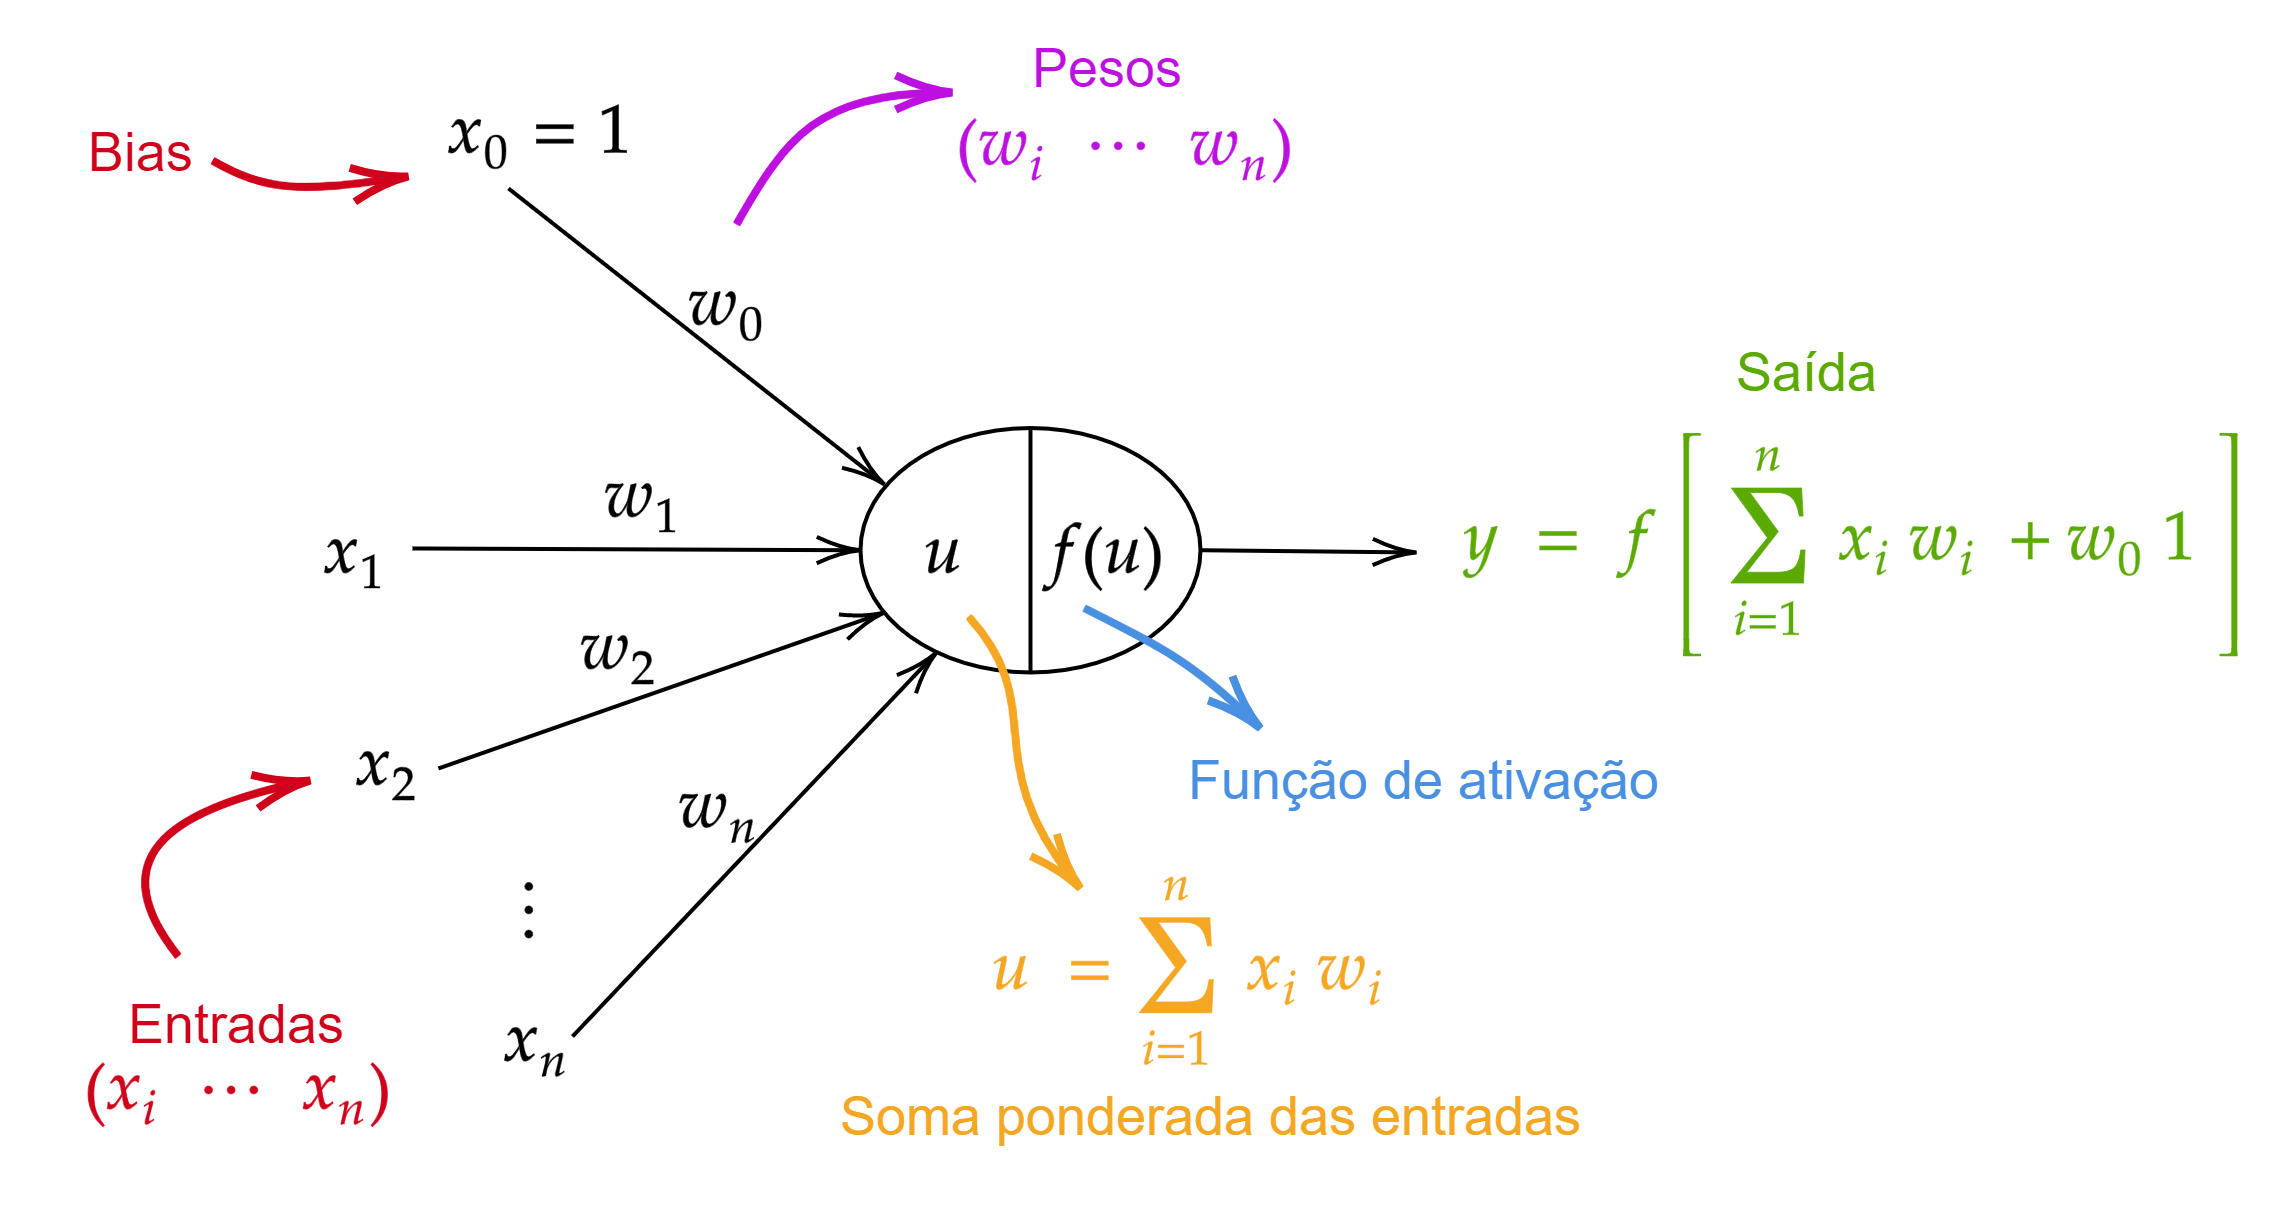
\includegraphics[scale=0.15]{Figuras/neuronio.png}
\end{figure}


\end{ftst}

%=====

\begin{ftst}{Funções de ativação}{Redes Neurais}

\textbf{Função degrau:} usada na camada de saída para problemas de classificação.
\begin{figure}
    \centering
    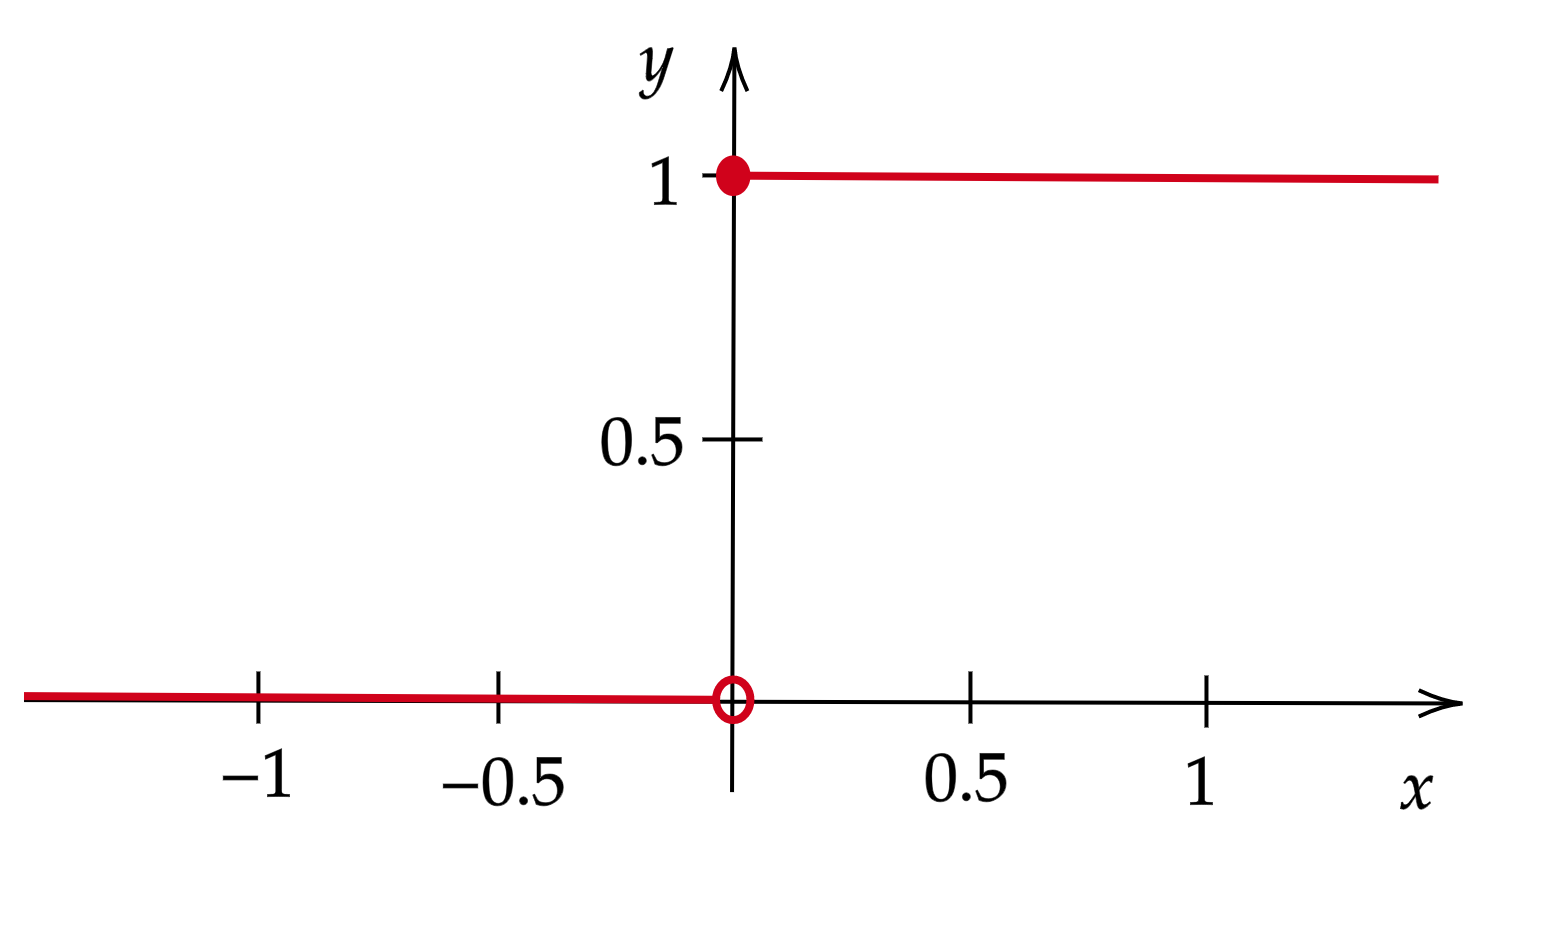
\includegraphics[scale=0.12]{Figuras/degrau.png}
\end{figure}

\begin{equation}
    f(u) = \left\{\begin{matrix} 
    1 & \text{se } u \geq 0\\ 0 & 
    \text{se } u < 0
    \end{matrix}\right.
\end{equation}


\end{ftst}

%=====

\begin{ftst}{Funções de ativação}{Redes Neurais}

\textbf{Função linear:} usada na camada de saída para problemas de regressão.
\begin{figure}[!htb]
    \centering
    \begin{minipage}{.5\textwidth}
        \centering
        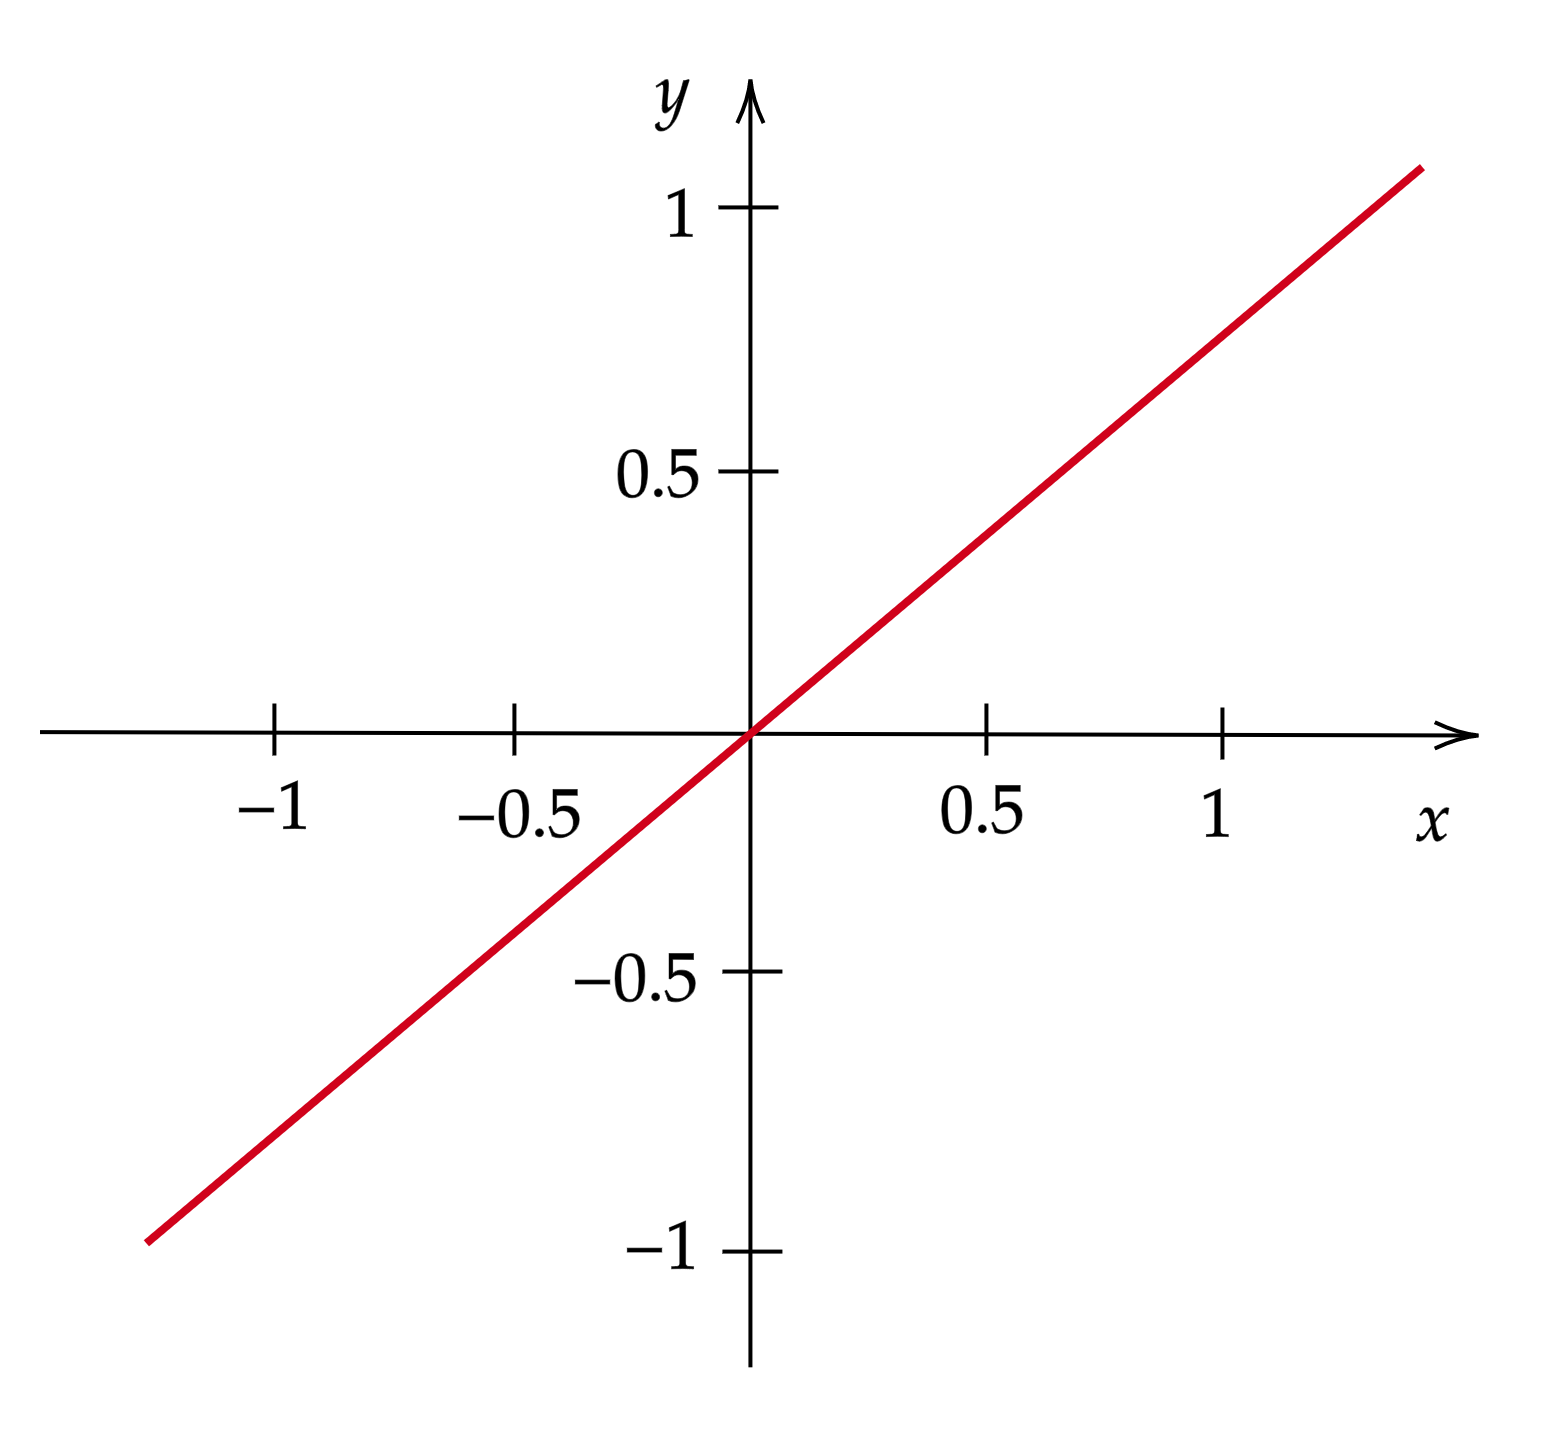
\includegraphics[scale=0.1]{Figuras/linear.png}
        \label{fig:prob1_6_2}
    \end{minipage}%
    \begin{minipage}{0.5\textwidth}
        \centering
        \begin{equation}
            f(u) = u
        \end{equation}
        \text{Intervalo:} \left [ -\infty, +\infty  \right ]
    \end{minipage}
\end{figure}
\end{ftst}

%=====

\begin{ftst}{Funções de ativação}{Redes Neurais}

\textbf{Função sigmóide:} usada na camada de saída para problemas de classificação binária.
\begin{figure}[!htb]
    \centering
    \begin{minipage}{.5\textwidth}
        \centering
        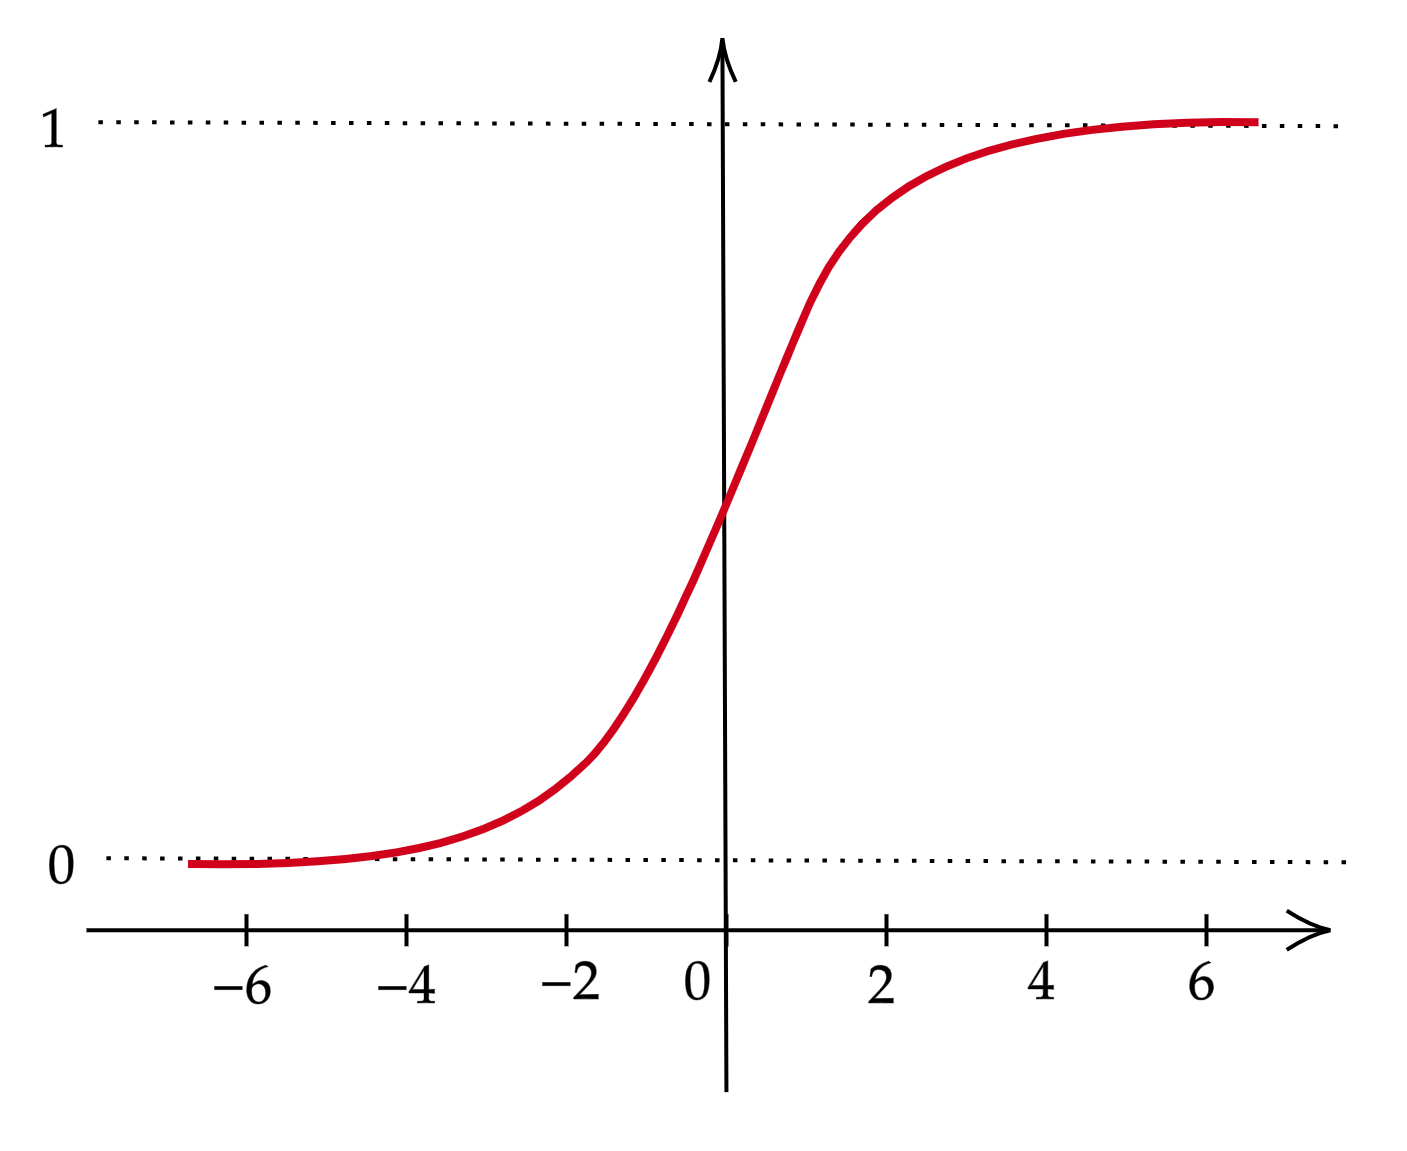
\includegraphics[scale=0.12]{Figuras/sigmoide.png}
        \label{fig:prob1_6_2}
    \end{minipage}%
    \begin{minipage}{0.5\textwidth}
        \centering
        \begin{equation}
            f(u) = \frac{1}{1+e^{-u}}
        \end{equation}
        \text{Intervalo:} \left [ 0, 1]
    \end{minipage}
\end{figure}
\end{ftst}

%=====

\begin{ftst}{Funções de ativação}{Redes Neurais}

\textbf{Função softmax:} usada na camada de saída para problemas de classificação multiclasse.
\begin{figure}[!htb]
    \centering
    \begin{minipage}{.5\textwidth}
        \centering
        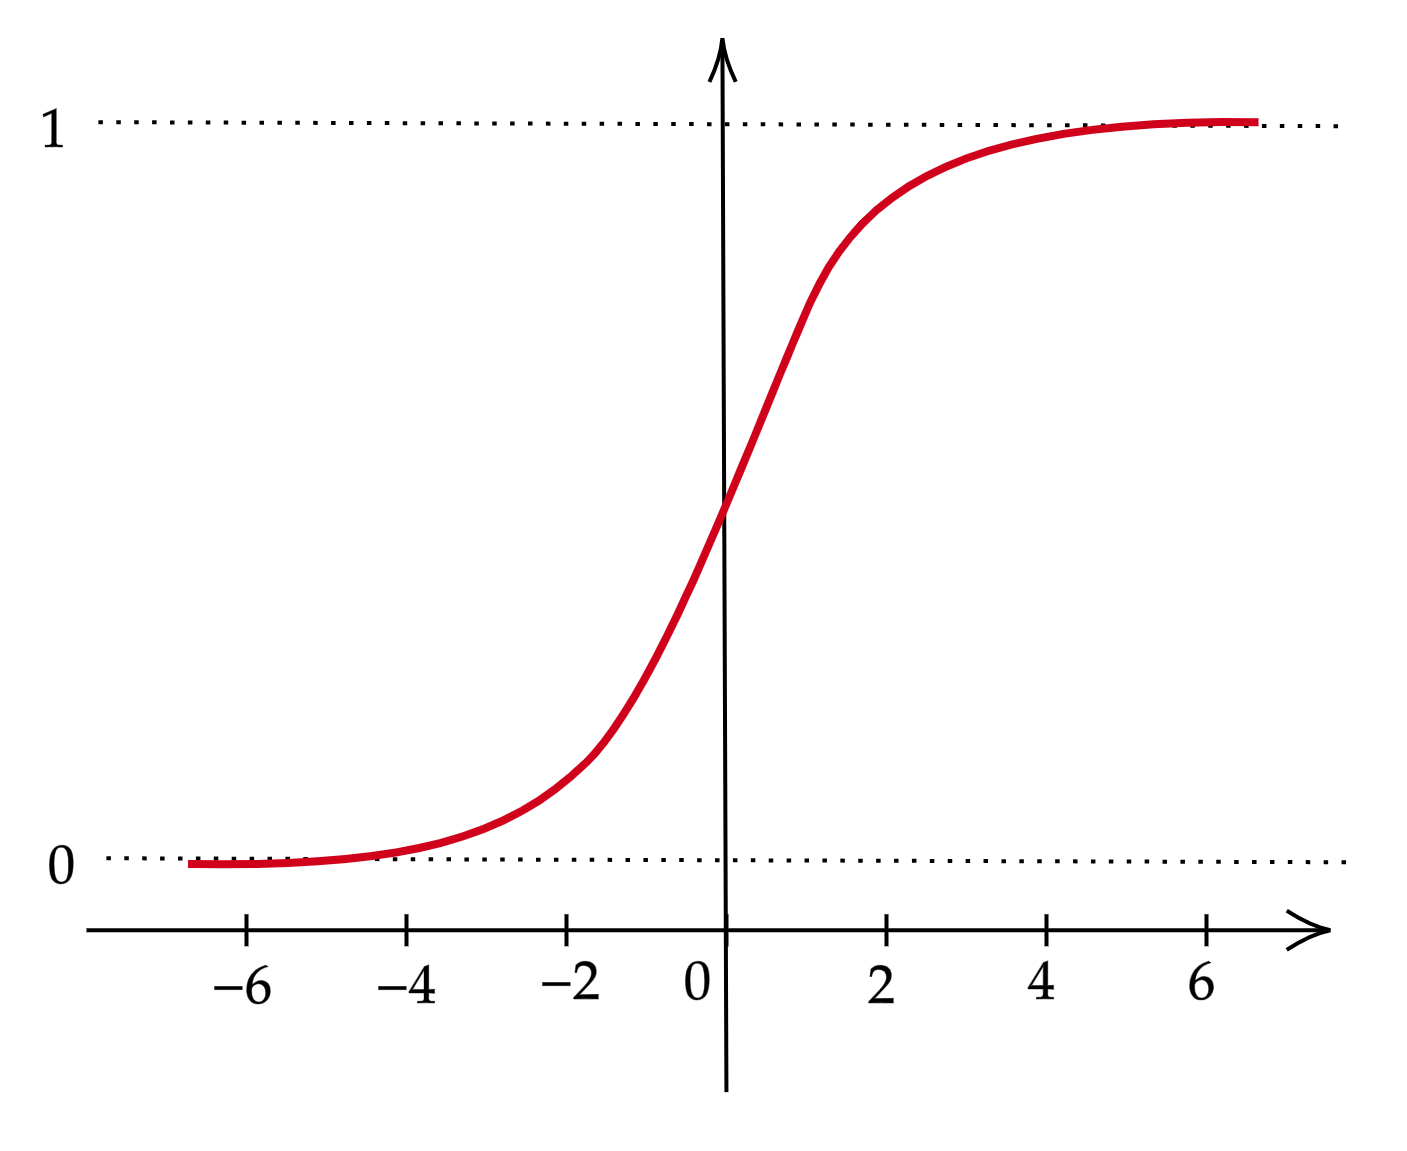
\includegraphics[scale=0.12]{Figuras/sigmoide.png}
        \label{fig:prob1_6_2}
    \end{minipage}%
    \begin{minipage}{0.5\textwidth}
        \centering
        \begin{equation}
            f(u) = \frac{e^{u_i}}{\sum e^{u_i}}
        \end{equation}
        \text{Intervalo:} \left [ 0, 1]
    \end{minipage}
\end{figure}
\end{ftst}

%=====

\begin{ftst}{Funções de ativação}{Redes Neurais}

\textbf{Função tangente hiperbólica:} usada na camada escondida.

\begin{figure}[!htb]
    \centering
    \begin{minipage}{.5\textwidth}
        \centering
        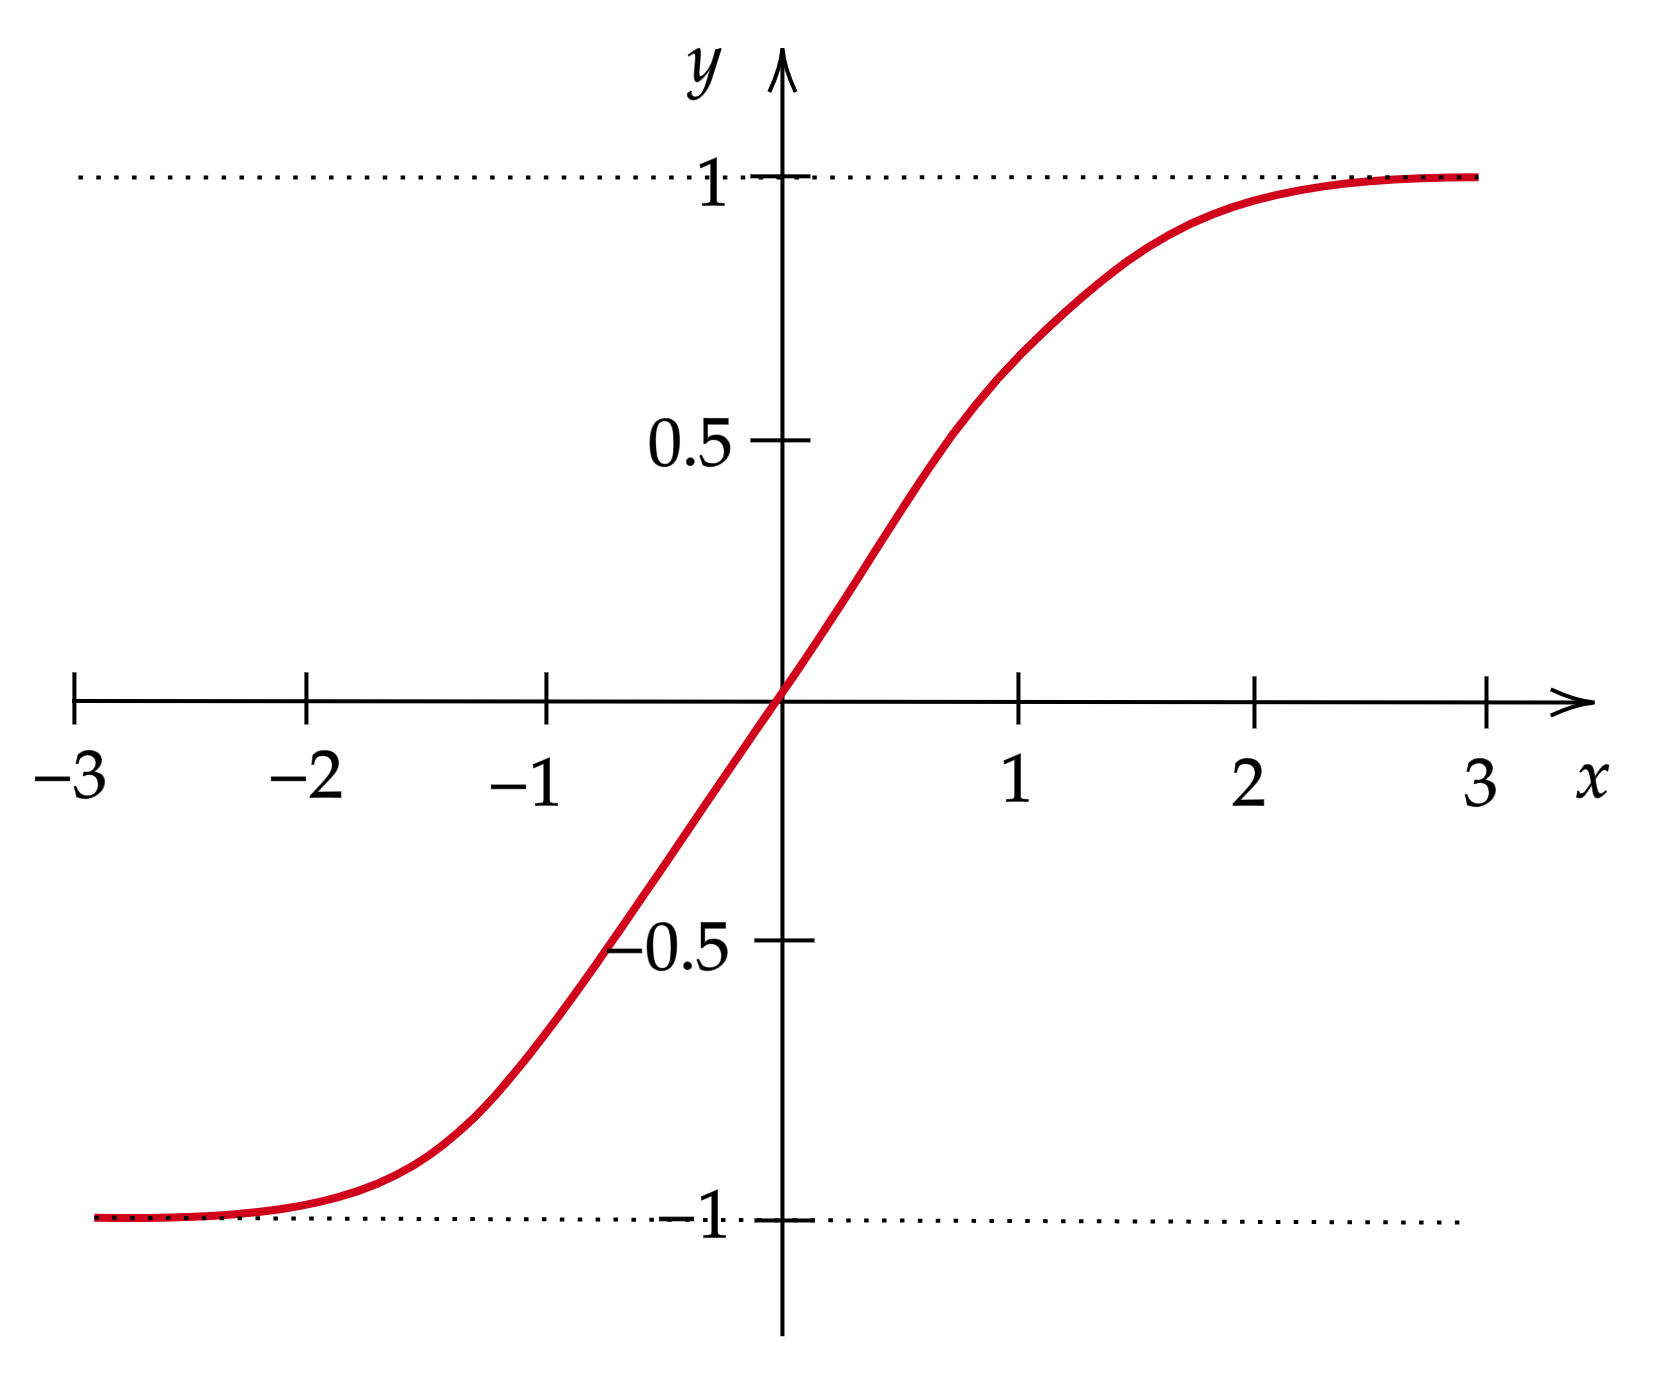
\includegraphics[scale=0.12]{Figuras/tanh.png}
        \label{fig:prob1_6_2}
    \end{minipage}%
    \begin{minipage}{0.5\textwidth}
        \centering
        \begin{equation}
            f(u) = \frac{e^{u}-e^{-u}}{e^{u}+e^{-u}}
        \end{equation}
        \text{Intervalo:} \left [ -1, 1]
    \end{minipage}
\end{figure}
\end{ftst}

%=====

\begin{ftst}{Funções de ativação}{Redes Neurais}

\textbf{Função Relu (unidade linear retificada):} usada na camada escondida.

\begin{figure}[!htb]
    \centering
    \begin{minipage}{.5\textwidth}
        \centering
        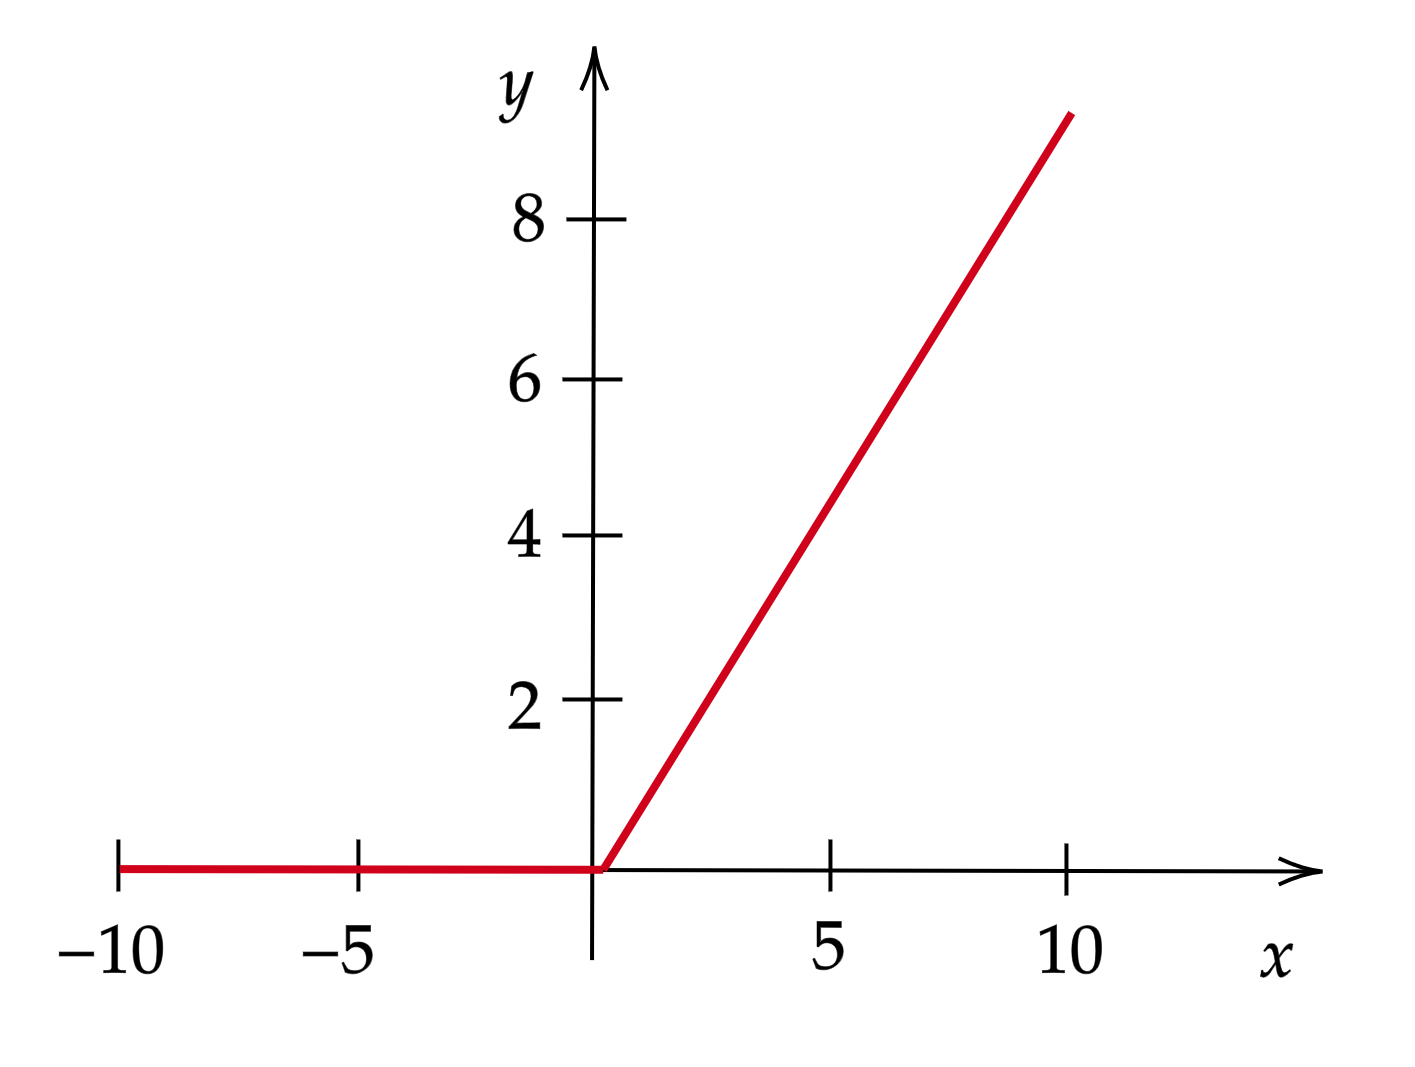
\includegraphics[scale=0.12]{Figuras/relu.png}
        \label{fig:prob1_6_2}
    \end{minipage}%
    \begin{minipage}{0.5\textwidth}
        \centering
        \begin{equation}
            f(u) = max(0,u)
        \end{equation}
        $f(u) = \left\{\begin{matrix} 
                0 & \text{se } u < 0\\ 
                u & \text{se } u \geq 0
                \end{matrix}\right.$
    \end{minipage}
\end{figure}
\end{ftst}

%=====

\begin{ftst}{Aprendizado supervisionado}{Redes Neurais}

Nesse tipo de aprendizado, os pesos são ajustados através da comparação da saída da rede com a saída desejada.
\vone
O método mais comum de aprendizado supervisionado é o aprendizado por correção de erros, em que procura-se minimizar o erro da resposta atual da rede em relação à saída desejada.
\vone
O erro:
\vone

\begin{equation}
    e = y - \hat{y}
\end{equation}

\end{ftst}

%=====

\begin{ftst}{Aprendizado supervisionado}{Redes Neurais}

Para a atualização dos pesos por correção dos erros usa-se a equação \ref{eq:regradacadeia}, chamada de Regra Delta:


\begin{equation}
    w_i(t+1) = w_i(t) + \eta e x_i 
    \label{eq:regradacadeia}
\end{equation}

onde:
\begin{itemize}
    \item $w_i(t+1)$ = novos pesos
    \item $w_i(t)$ = pesos atuais
    \item $\eta$ = taxa de aprendizagem
    \item $e$ = erro
    \item $x_i$ = entradas
\end{itemize}

\end{ftst}

%===

\begin{ftst}{Perceptron}{Redes Neurais}

O perceptron é uma rede neural de camada única que resolve problemas de classificação linear (binária).
\begin{figure}
    \centering
    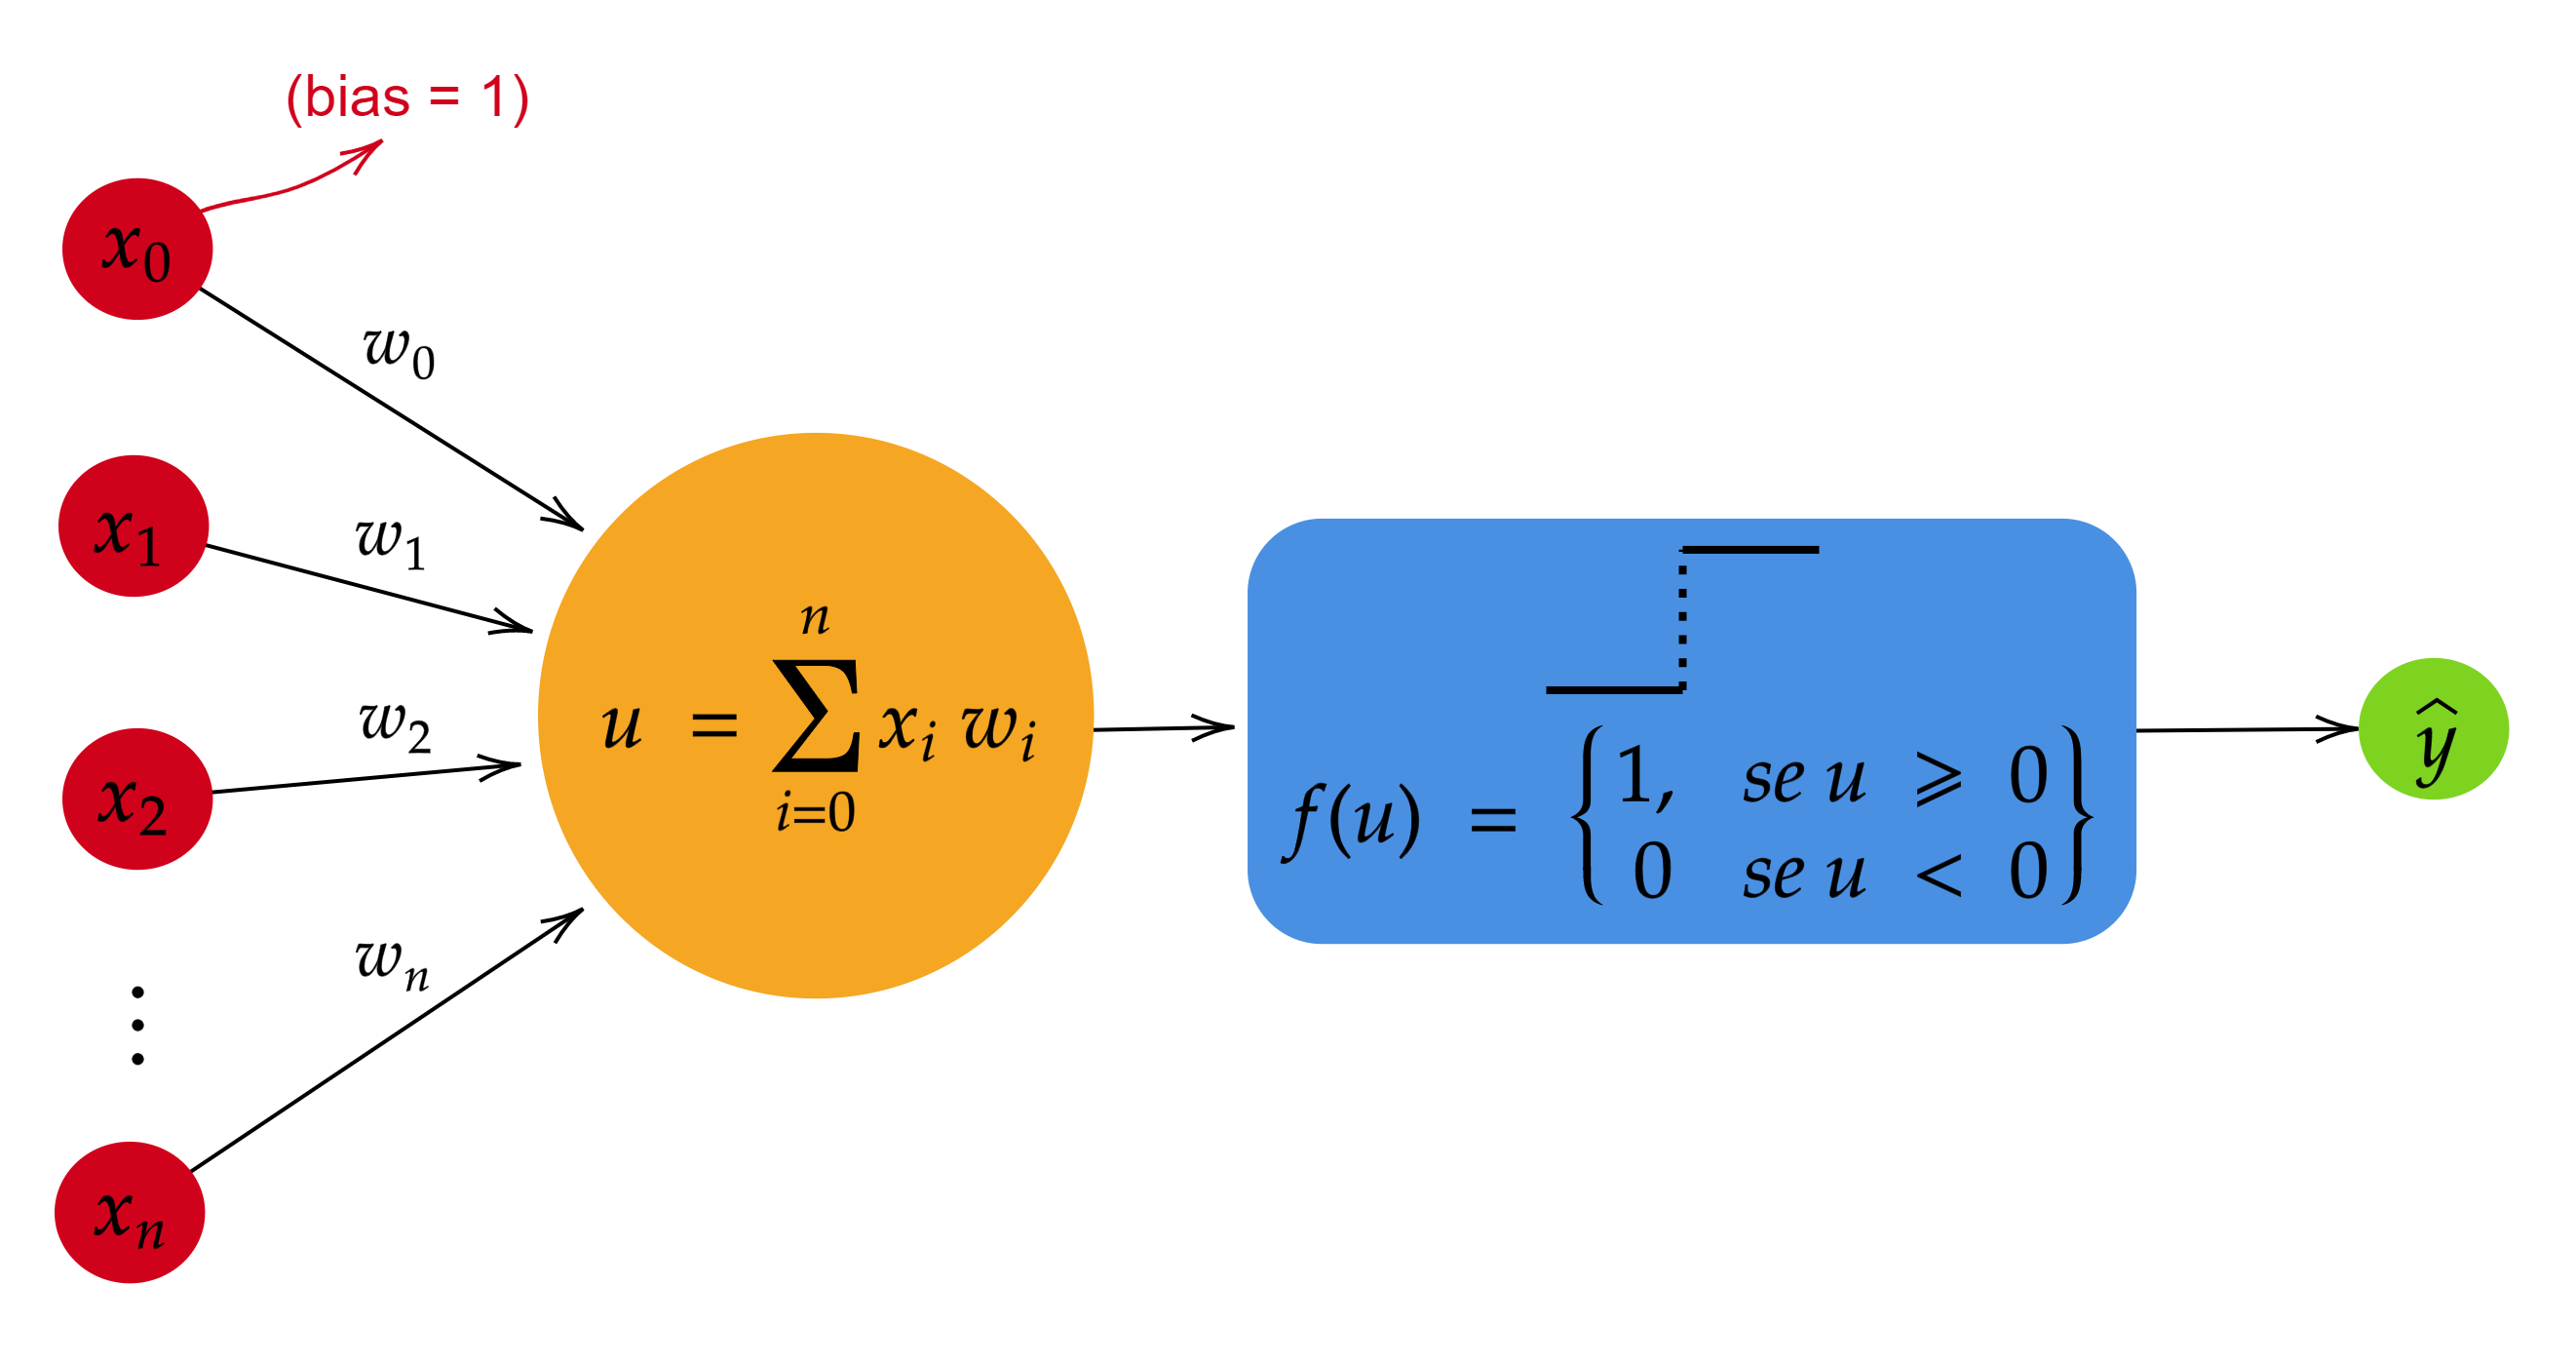
\includegraphics[scale=0.12]{Figuras/perceptron.png}
    \label{fig:perceptron}
\end{figure}

\end{ftst}

%===

\begin{ftst}{O algoritmo Perceptron}{Redes Neurais}
\begin{itemize}
    \item[1.] Inicializar $\eta$
    \item[2.] Inicializar os pesos $w$ com valores aleatórios
    \item[3.] Repita até $\sum e^2 = 0$
    
    \setlength{\leftskip}{1cm}
        \item[3.1] Calcule $f(u)$
        \item[3.2] Calcule $e$
        \item[3.3] Aplique a regra de atualização dos pesos para todos os pares $(x_i,y_i)$ do conjunto de treinamento
        \item[3.4] Calcule $\sum e^2$

\end{itemize}


\end{ftst}

%===

\begin{ftst}{Algumas considerações...}{Redes Neurais}
\begin{figure}[!htb]
    \centering
    \begin{minipage}{.5\textwidth}
        \footnotesize
        \begin{itemize}
        \item Valor da taxa de aprendizado ($\eta$): valores muito pequenos podem levar a um tempo de convergência muito alto, enquanto que valores muito altos podem levar a instabilidade no treinamento.
        \item Inicialização dos pesos: em geral devem ser inicializados com valores no intervalo $[-0.5,0.5]$.
        \item Normalizar e embaralhar as entradas.
\end{itemize}
    \end{minipage}%
    \begin{minipage}{0.5\textwidth}
        \centering
        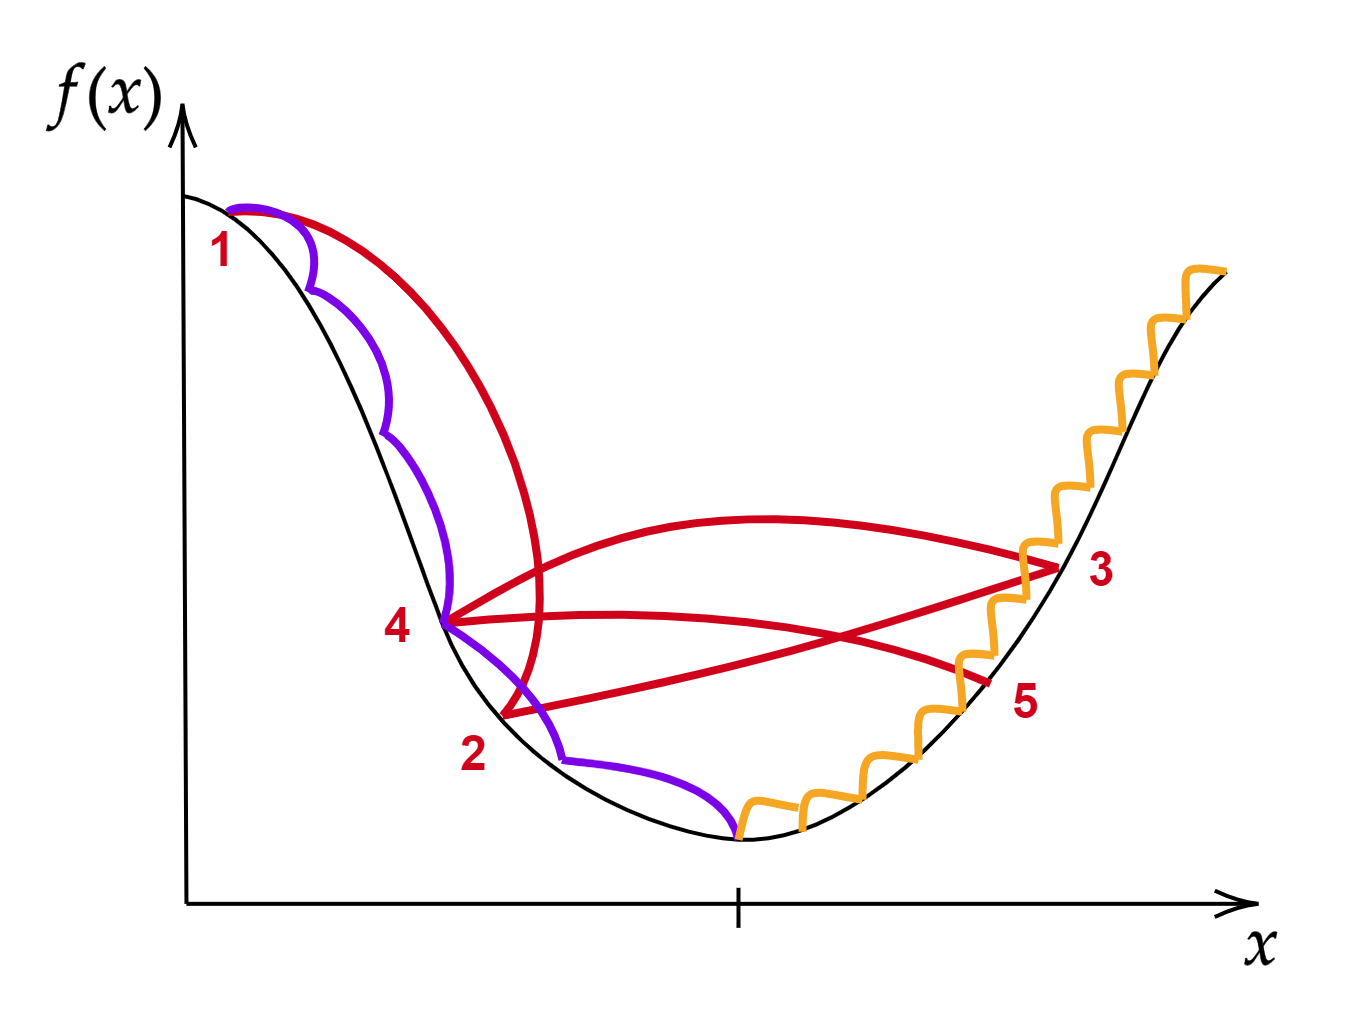
\includegraphics[scale=0.12]{Figuras/learning_rate.png}
    \end{minipage}
\end{figure}

\end{ftst}

%===

\begin{ftst}{Adaline}{Redes Neurais}
O adaline é uma rede neural de camada única que resolve problemas de regressão.

\begin{figure}
    \centering
    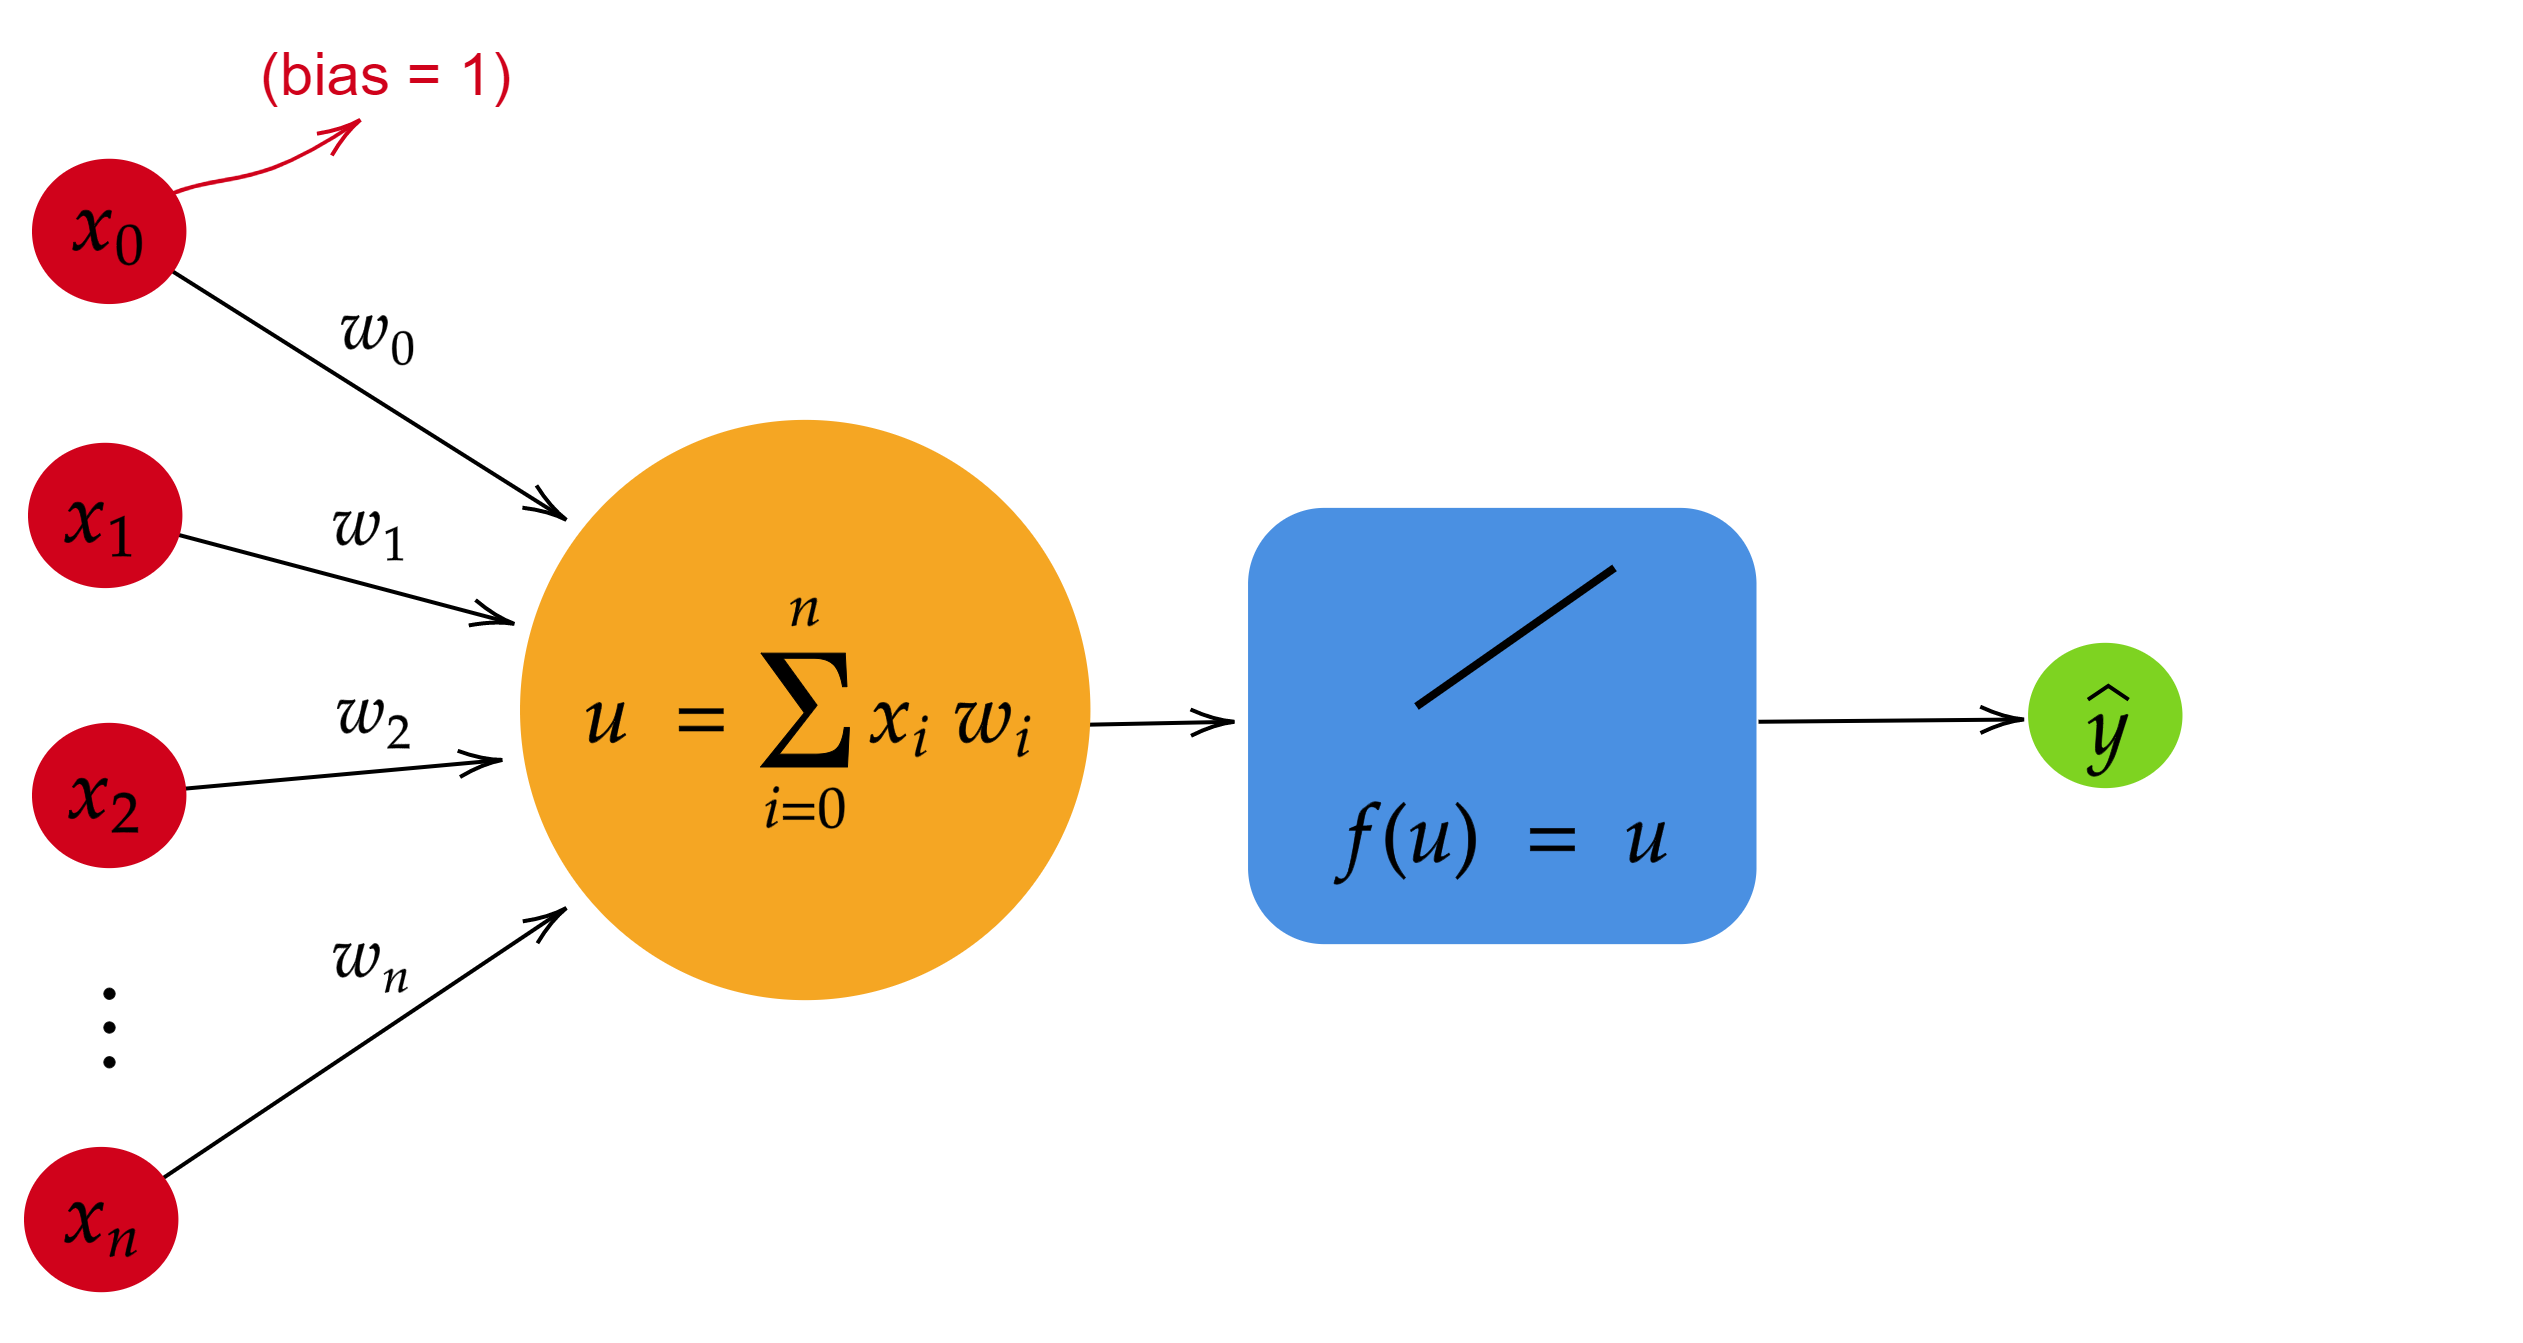
\includegraphics[scale=0.12]{Figuras/adaline.png}
    \label{fig:perceptron}
\end{figure}

\end{ftst}

%===

\begin{ftst}{Perceptron de múltiplas camadas - MLP}{Redes Neurais}
\footnotesize
\begin{itemize}
    \item As redes vista até aqui, com uma única camada, têm a limitação de resolver apenas problemas com características lineares.
    \begin{figure}
        \centering
        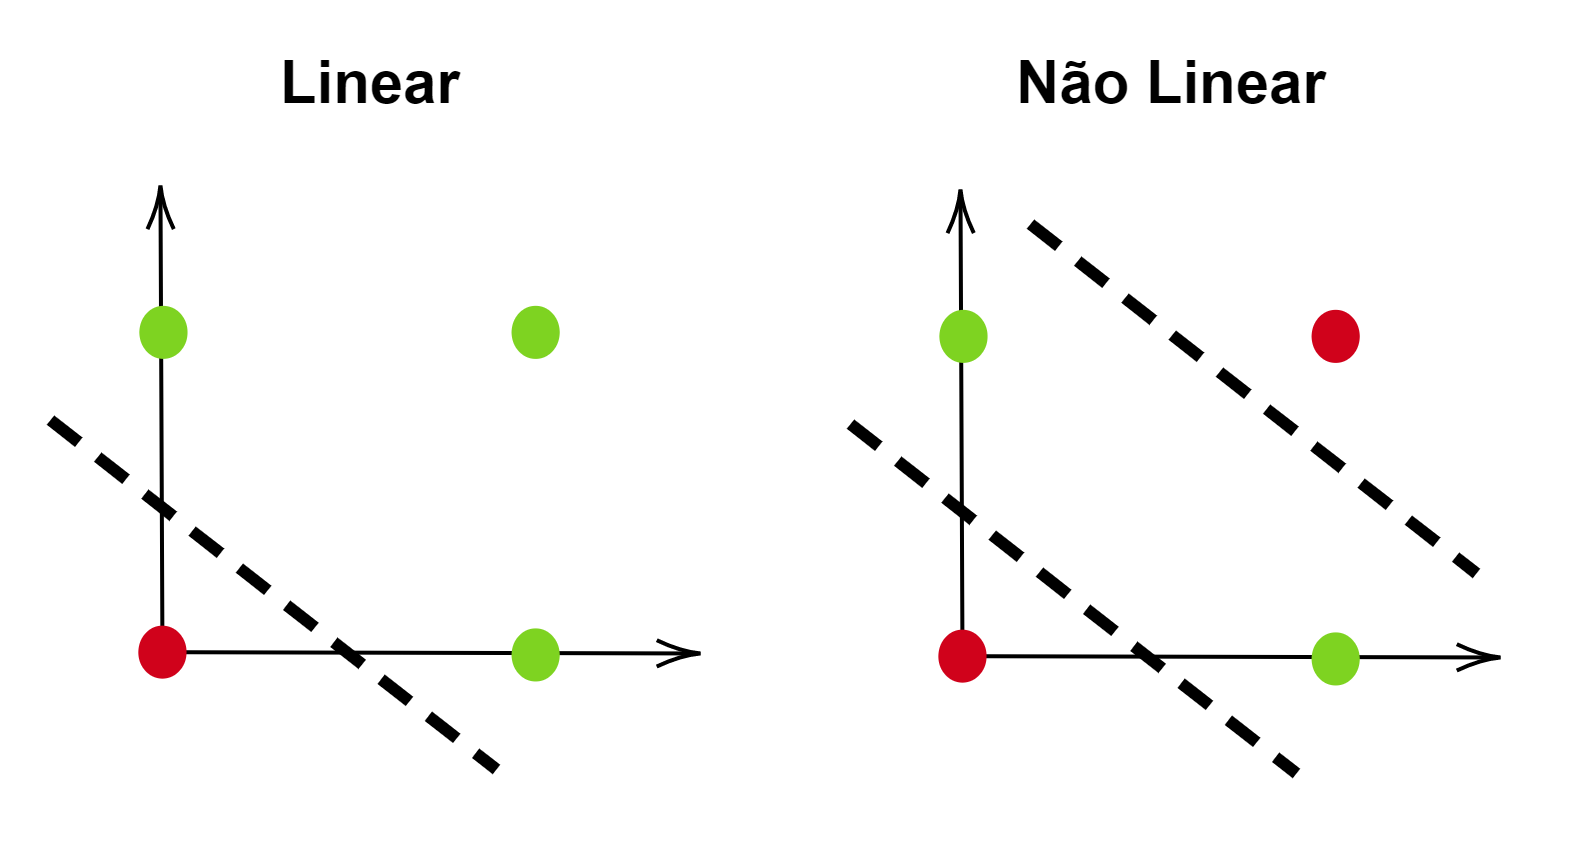
\includegraphics[scale=0.1]{Figuras/nolinear.png}
    \end{figure}
    \item No entanto, a não-linearidade é inerente à maioria das situações e problemas reais, sendo necessária a utilização de estruturas com características não-lineares para resolução de problemas de maior complexidade.
    \vone
    \item As não-linearidades são incorporadas a modelos neurais através das funções de ativação (não-lineares) de cada neurônio da rede e da composição da sua estrutura em camadas sucessivas.
\end{itemize}

\end{ftst}

%===

\begin{ftst}{Perceptron de múltiplas camadas - MLP}{Redes Neurais}
\textbf{Arquitetura:}
o comportamento de uma MLP com 1 camada intermediária, pode ser descrito por meio de duas transformações sucessivas:
    \begin{equation}
        Y(H(x,w_i),w_s)
    \end{equation}
    \scriptsize
onde:
    \begin{itemize}
        \item $w_i$ são os pesos da camada intermediária.
        \item $w_s$ são os pesos da camada de saída.
    \end{itemize}
    
\begin{figure}
    \centering
    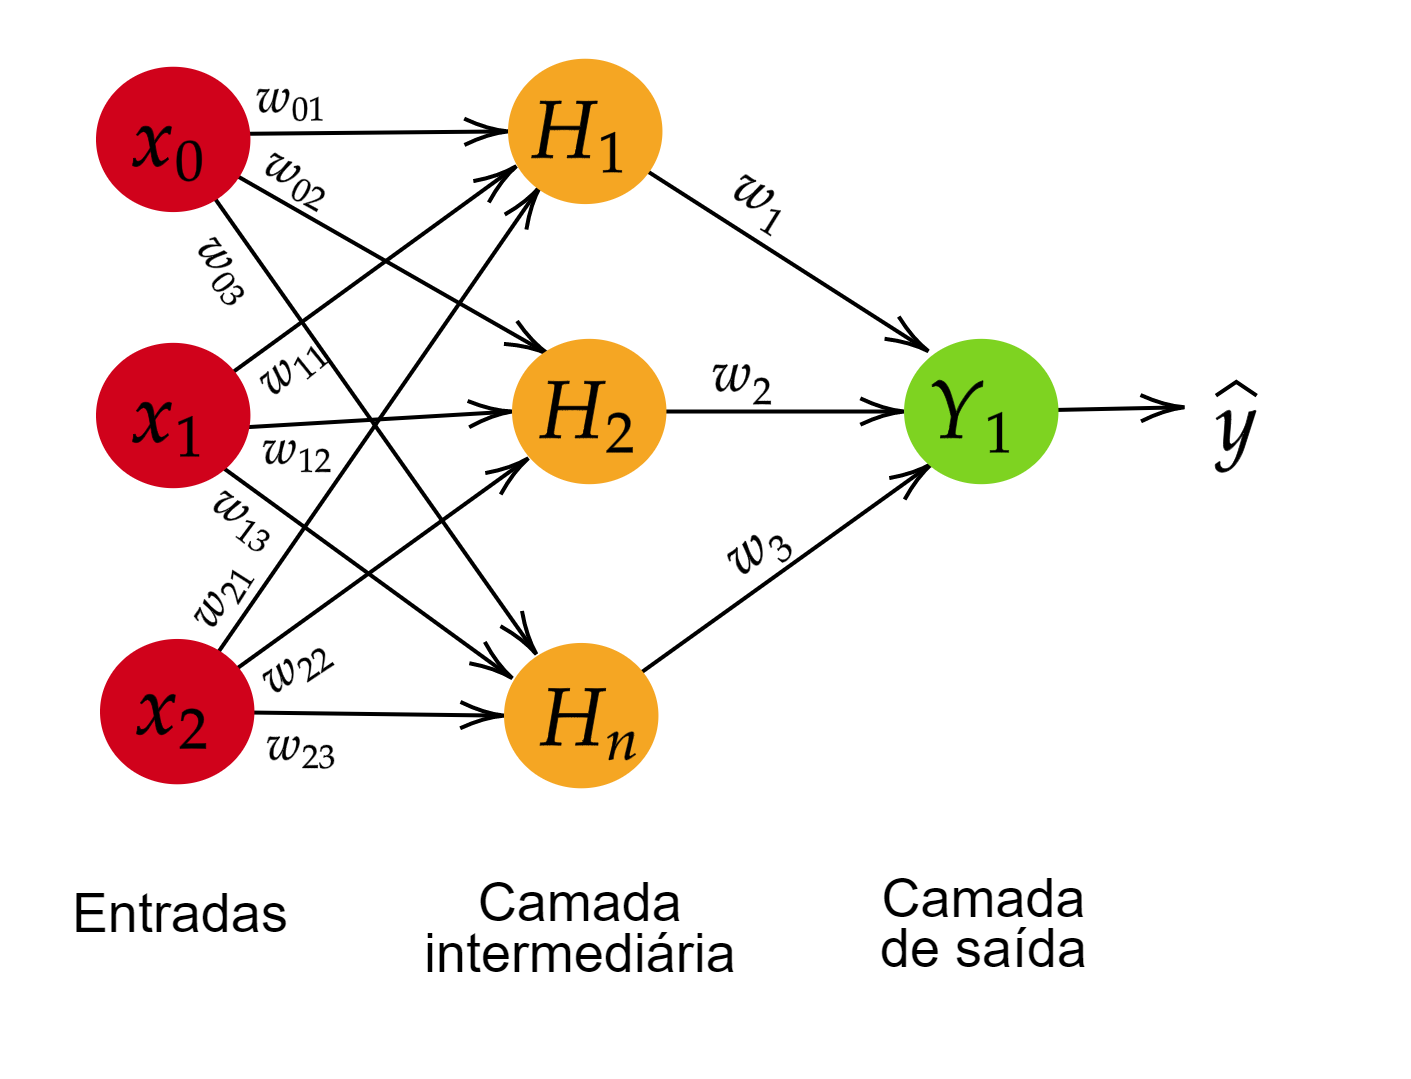
\includegraphics[scale=0.13]{Figuras/mlp.png}
\end{figure}

\end{ftst}

%===

\begin{ftst}{Perceptron de múltiplas camadas - MLP}{Redes Neurais}
\textbf{Número de camadas:}
\vone

\begin{figure}
    \centering
    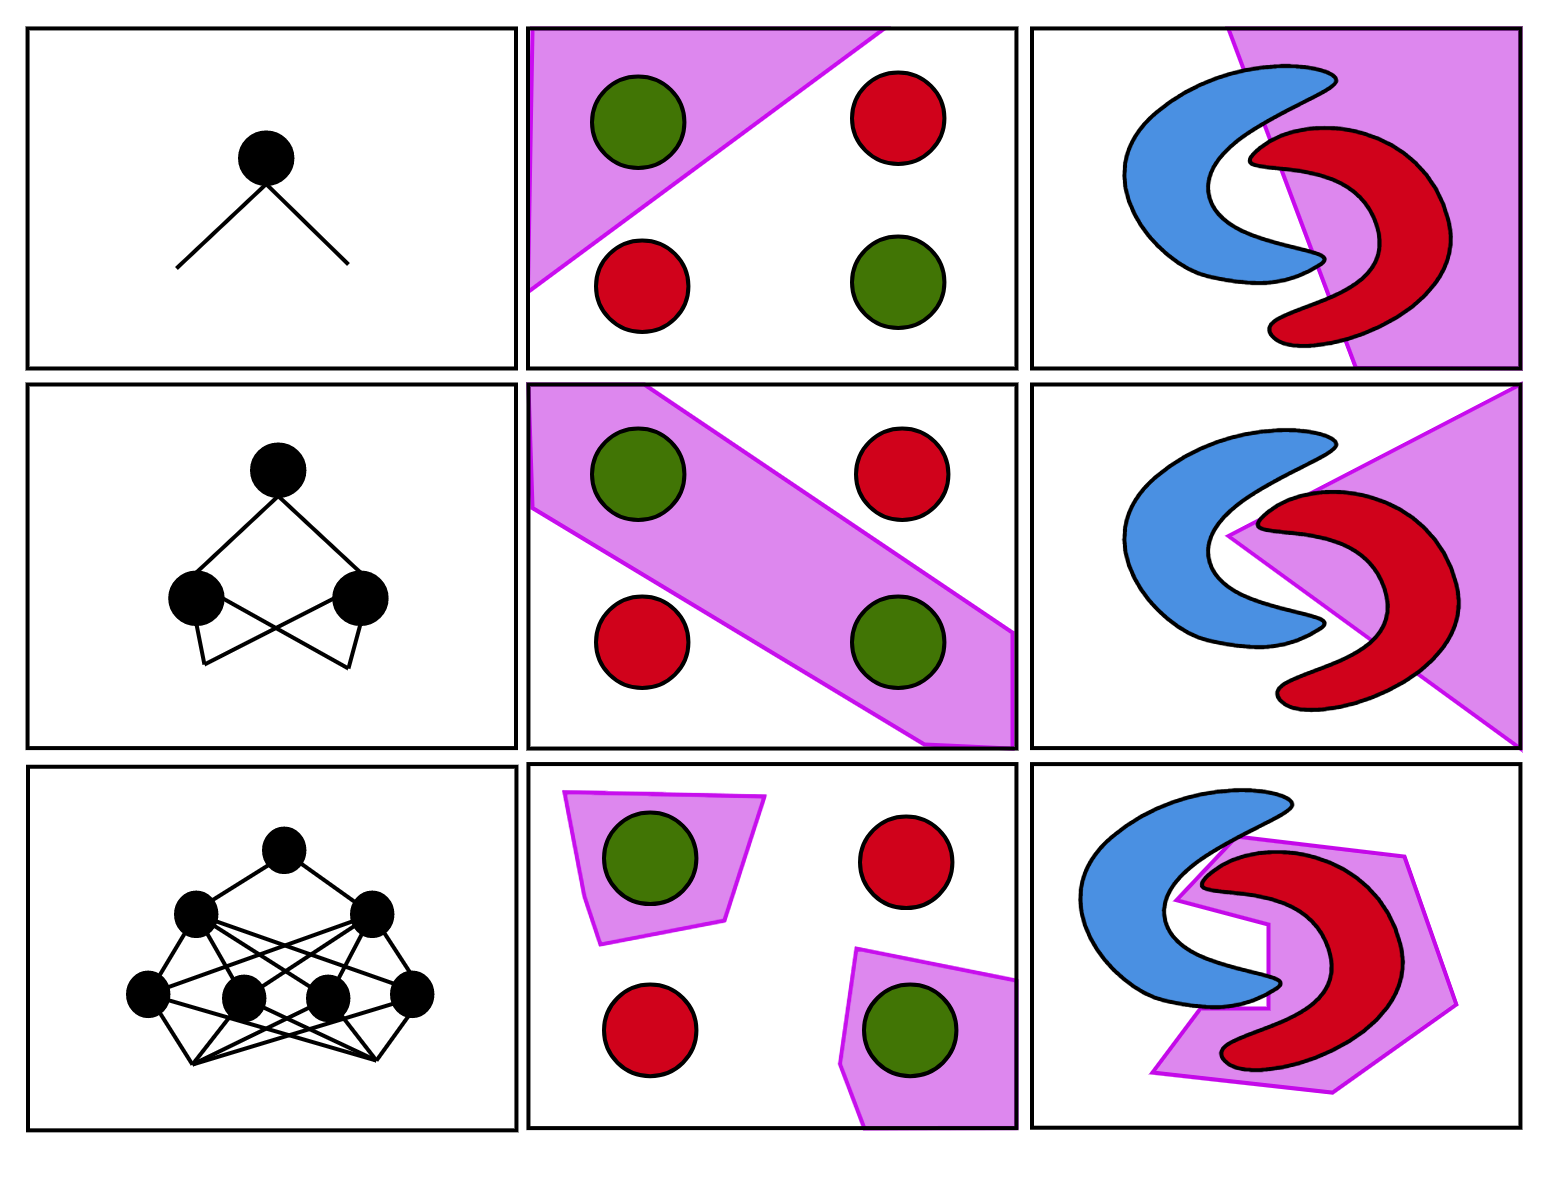
\includegraphics[scale=0.15]{Figuras/regioes.png}
\end{figure}

\end{ftst}

%===

\begin{ftst}{Perceptron de múltiplas camadas - MLP}{Redes Neurais}
\textbf{Número de neurônios:}
\vone
\begin{itemize}
    \item O número de neurônios determina a capacidade da rede em resolver problemas de determinada complexidade. 
    \item Quanto maior o número de neurônios, maior a complexidade da rede e maior a sua abrangência em termos de soluções possíveis.
    \item A determinação do número de neurônios é o problema mais fundamental em aprendizado de redes neurais, mas ainda não existe uma regra geral para resolvê-lo.
\end{itemize}

\end{ftst}

%===

\begin{ftst}{Perceptron de múltiplas camadas - MLP}{Redes Neurais}
O treinamento de redes de uma única camada por meio do aprendizado supervisionado e correção de erros é realizado através da equação:

\begin{equation}
    w_i(t+1) = w_i(t) + \eta e x_i
\end{equation}

\begin{equation}
    e = y - \hat{y}
\end{equation}

No entanto, para redes de múltiplas camadas esse procedimento pode ser aplicado somente na camada de saída, já que não existem saídas desejadas nas camadas intermediárias!


\end{ftst}

%===

\begin{ftst}{Perceptron de múltiplas camadas - MLP}{Redes Neurais}
\textbf{Solução:} algoritmo de retropropagação de erros (back-propagation).
\vone
\begin{itemize}
    \item O princípio desse algoritmo é, utilizando-se do gradiente descendente, estimar o erro das camadas intermediárias por meio de uma estimativa do efeito que estas causam no erro da camada de saída.
    \item Assim, o erro de saída da rede é calculado e este é retroalimentado para as camadas intermediárias, possibilitando o ajuste dos pesos proporcionalmente aos valores das conexões entre as camadas.
    \item Requer o uso de funções de ativação contínuas e diferenciáveis.

\end{itemize}


\end{ftst}

%===



\end{document}